\subsection{Learning $\nfhef$}

We now describe a learning algorithm for $\nfhef$.
Our algorithm is based on Angluin's $L^*$ algorithm \cite{Angluin87} for regular languages, and aims to learn a minimal deterministic permutation-sequence complete $\nfhef$ with a minimal number of variables for a hyperlanguage $\cal L$.

As with $L^*$, our algorithm consists of two entities: a {\em learner} and a {\em teacher}.
During the learning process, the learner asks the teacher two types of queries: {\em membership queries} (``is the hyperword $S$ in $\cal L$?'') and {\em equivalence queries} (``Is $\A$ an $\nfhef$ for $\cal L$?'').


The number of variables, as well as the quantification condition $\alpha$, is unknown to the learner in advance, and is established during the learning procedure. 
In every step, the learner may cause one of the following to occur in the $\nfhef$ $\A$ that it maintains:
\begin{enumerate}
    \item Increase the number of states;
    \item Increase the number of variables;
    \item Turn an $\exists$ quantifier to a $\forall$ quantifier.
\end{enumerate}

As with $L^*$, the learner maintains an {\em observation table} $T$, which, intuitively, maintains the states and transitions of the underlying automaton that have been learned so far. In addition, the learner maintains the current number of variables $k$ (which also influences the alphabet of the observation table), and the number of $\exists$ quantifiers $t$ in the quantification condition. 

In case of a failed equivalence query, the teacher returns a {\em counterexample}: a {\em negative counterexample} is a hyperword that is not in $\lang{\A}$ and is in $\cal L$, and a {\em positive counterexample} is a hyperword that is in $\lang{\A}$, but is not in $\cal L$. We assume that the teacher always returns a minimal counterexample (in terms of set size).

The actions of the learner depend on the properties of the returned counterexample $S$ it gets from the teacher. 
We say that $S$ is {\em manifested} in $T$ if there exists a word $w$ in $T$ that is formed by zipping the words in $S$ in some order.
\begin{enumerate}
    \item 
    If $S$ is a positive counterexample of size $k$ or less, that is not manifested in $T$, then the learner adds  $\zip(S)$ to $T$, where $\zip(S)$ denotes zipping the words in $S$ in some arbitrary order. 
    \item 
    If $S$ is a positive counterexample of size $k$ or less, that is manifested in $T$, then the learner sets $t\leftarrow t-1$. 
    \item
    If $S$ is a positive counterexample of size $k'>k$, then the learner replaces every letter $\sigma$ in the transitions with $\uparrow^{k'}(\sigma)$, and sets $t\leftarrow t+(k'-k)$. 
    \item If $S$ is a negative counterexample, and $k>t$. then it must be that $S$ is of size $k$ or less, and does not already appear in $T$. The learner then adds $S$ to $T$.
    \item if $S$ is a negative counterexample of size $k'>k$, and $k=t$ (that is, the quantifiers are all $\exists$), then the learner sets $t\leftarrow t-1$.  
\end{enumerate}





\tikzset{every picture/.style={line width=0.75pt}} %set default line width to 0.75pt        

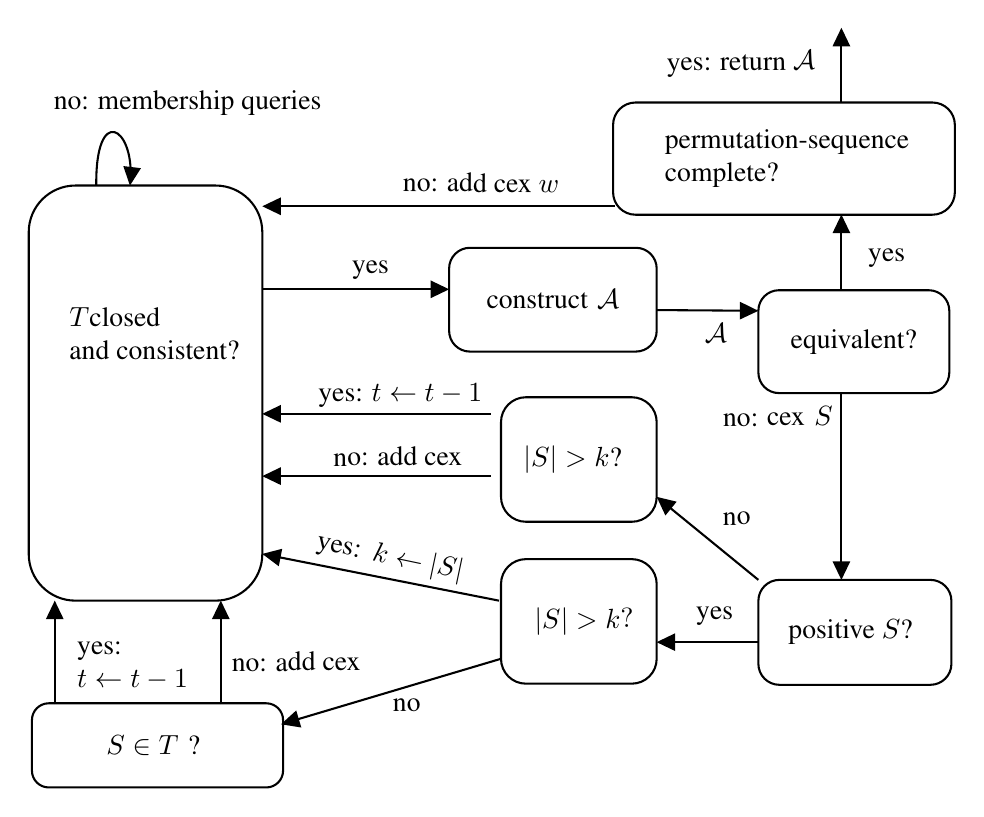
\begin{tikzpicture}[x=0.75pt,y=0.75pt,yscale=-1,xscale=1]
%uncomment if require: \path (0,427.3333320617676); %set diagram left start at 0, and has height of 427.3333320617676

%Curve Lines [id:da3319849647811628] 
\draw    (120,90) .. controls (119.52,50.76) and (138.13,61.49) .. (136.48,87.15) ;
\draw [shift={(136.22,90)}, rotate = 276.77] [fill={rgb, 255:red, 0; green, 0; blue, 0 }  ][line width=0.08]  [draw opacity=0] (8.93,-4.29) -- (0,0) -- (8.93,4.29) -- cycle    ;

%Rounded Rect [id:dp3318135503338837] 
\draw   (369,60.81) .. controls (369,54.84) and (373.84,50) .. (379.81,50) -- (522.85,50) .. controls (528.82,50) and (533.66,54.84) .. (533.66,60.81) -- (533.66,93.25) .. controls (533.66,99.22) and (528.82,104.06) .. (522.85,104.06) -- (379.81,104.06) .. controls (373.84,104.06) and (369,99.22) .. (369,93.25) -- cycle ;
%Straight Lines [id:da9118196858913674] 
\draw    (479,140) -- (479,107) ;
\draw [shift={(479,104)}, rotate = 450] [fill={rgb, 255:red, 0; green, 0; blue, 0 }  ][line width=0.08]  [draw opacity=0] (8.93,-4.29) -- (0,0) -- (8.93,4.29) -- cycle    ;

%Rounded Rect [id:dp46825370670489375] 
\draw   (439,290.11) .. controls (439,284.53) and (443.53,280) .. (449.11,280) -- (521.89,280) .. controls (527.47,280) and (532,284.53) .. (532,290.11) -- (532,320.44) .. controls (532,326.02) and (527.47,330.55) .. (521.89,330.55) -- (449.11,330.55) .. controls (443.53,330.55) and (439,326.02) .. (439,320.44) -- cycle ;
%Rounded Rect [id:dp8177115097200811] 
\draw   (87.45,112.51) .. controls (87.45,100.08) and (97.53,90) .. (109.96,90) -- (177.49,90) .. controls (189.92,90) and (200,100.08) .. (200,112.51) -- (200,267.49) .. controls (200,279.92) and (189.92,290) .. (177.49,290) -- (109.96,290) .. controls (97.53,290) and (87.45,279.92) .. (87.45,267.49) -- cycle ;
%Straight Lines [id:da13258260836721147] 
\draw    (479,190) -- (479,277) ;
\draw [shift={(479,280)}, rotate = 270] [fill={rgb, 255:red, 0; green, 0; blue, 0 }  ][line width=0.08]  [draw opacity=0] (8.93,-4.29) -- (0,0) -- (8.93,4.29) -- cycle    ;

%Straight Lines [id:da907821786011709] 
\draw    (439,310) -- (393,310) ;
\draw [shift={(390,310)}, rotate = 360] [fill={rgb, 255:red, 0; green, 0; blue, 0 }  ][line width=0.08]  [draw opacity=0] (8.93,-4.29) -- (0,0) -- (8.93,4.29) -- cycle    ;

%Straight Lines [id:da6213919327201678] 
\draw    (100,340) -- (100,293) ;
\draw [shift={(100,290)}, rotate = 450] [fill={rgb, 255:red, 0; green, 0; blue, 0 }  ][line width=0.08]  [draw opacity=0] (8.93,-4.29) -- (0,0) -- (8.93,4.29) -- cycle    ;

%Rounded Rect [id:dp20293608518691664] 
\draw   (315,204) .. controls (315,197.37) and (320.37,192) .. (327,192) -- (378,192) .. controls (384.63,192) and (390,197.37) .. (390,204) -- (390,240) .. controls (390,246.63) and (384.63,252) .. (378,252) -- (327,252) .. controls (320.37,252) and (315,246.63) .. (315,240) -- cycle ;
%Straight Lines [id:da026165564694643928] 
\draw    (200,140) -- (287,140) ;
\draw [shift={(290,140)}, rotate = 180] [fill={rgb, 255:red, 0; green, 0; blue, 0 }  ][line width=0.08]  [draw opacity=0] (8.93,-4.29) -- (0,0) -- (8.93,4.29) -- cycle    ;

%Straight Lines [id:da7822788939849978] 
\draw    (390,150) -- (436,150.33) ;
\draw [shift={(439,150.35)}, rotate = 180.41] [fill={rgb, 255:red, 0; green, 0; blue, 0 }  ][line width=0.08]  [draw opacity=0] (8.93,-4.29) -- (0,0) -- (8.93,4.29) -- cycle    ;

%Straight Lines [id:da6722982390392582] 
\draw    (439,280) -- (392.32,241.9) ;
\draw [shift={(390,240)}, rotate = 399.23] [fill={rgb, 255:red, 0; green, 0; blue, 0 }  ][line width=0.08]  [draw opacity=0] (8.93,-4.29) -- (0,0) -- (8.93,4.29) -- cycle    ;

%Straight Lines [id:da02752677732389186] 
\draw    (180,340) -- (180,293) ;
\draw [shift={(180,290)}, rotate = 450] [fill={rgb, 255:red, 0; green, 0; blue, 0 }  ][line width=0.08]  [draw opacity=0] (8.93,-4.29) -- (0,0) -- (8.93,4.29) -- cycle    ;

%Rounded Rect [id:dp47353225212057115] 
\draw   (439,150.35) .. controls (439,144.88) and (443.44,140.44) .. (448.91,140.44) -- (521.07,140.44) .. controls (526.55,140.44) and (530.99,144.88) .. (530.99,150.35) -- (530.99,180.09) .. controls (530.99,185.56) and (526.55,190) .. (521.07,190) -- (448.91,190) .. controls (443.44,190) and (439,185.56) .. (439,180.09) -- cycle ;
%Rounded Rect [id:dp263772512188744] 
\draw   (290,130) .. controls (290,124.48) and (294.48,120) .. (300,120) -- (380,120) .. controls (385.52,120) and (390,124.48) .. (390,130) -- (390,160) .. controls (390,165.52) and (385.52,170) .. (380,170) -- (300,170) .. controls (294.48,170) and (290,165.52) .. (290,160) -- cycle ;
%Rounded Rect [id:dp6512928292961364] 
\draw   (315,282) .. controls (315,275.37) and (320.37,270) .. (327,270) -- (378,270) .. controls (384.63,270) and (390,275.37) .. (390,282) -- (390,318) .. controls (390,324.63) and (384.63,330) .. (378,330) -- (327,330) .. controls (320.37,330) and (315,324.63) .. (315,318) -- cycle ;
%Straight Lines [id:da09911735351490747] 
\draw    (310,230) -- (203,230) ;
\draw [shift={(200,230)}, rotate = 360] [fill={rgb, 255:red, 0; green, 0; blue, 0 }  ][line width=0.08]  [draw opacity=0] (8.93,-4.29) -- (0,0) -- (8.93,4.29) -- cycle    ;

%Rounded Rect [id:dp3802867081039123] 
\draw   (89,347.56) .. controls (89,343.08) and (92.63,339.45) .. (97.11,339.45) -- (201.89,339.45) .. controls (206.37,339.45) and (210,343.08) .. (210,347.56) -- (210,371.89) .. controls (210,376.37) and (206.37,380) .. (201.89,380) -- (97.11,380) .. controls (92.63,380) and (89,376.37) .. (89,371.89) -- cycle ;
%Straight Lines [id:da8300687346036015] 
\draw    (310,200) -- (203,200) ;
\draw [shift={(200,200)}, rotate = 360] [fill={rgb, 255:red, 0; green, 0; blue, 0 }  ][line width=0.08]  [draw opacity=0] (8.93,-4.29) -- (0,0) -- (8.93,4.29) -- cycle    ;

%Straight Lines [id:da8484446028025674] 
\draw    (314,290) -- (202.94,268.07) ;
\draw [shift={(200,267.49)}, rotate = 371.16999999999996] [fill={rgb, 255:red, 0; green, 0; blue, 0 }  ][line width=0.08]  [draw opacity=0] (8.93,-4.29) -- (0,0) -- (8.93,4.29) -- cycle    ;

%Straight Lines [id:da1736308020815165] 
\draw    (315,318) -- (211.88,348.7) ;
\draw [shift={(209,349.56)}, rotate = 343.41999999999996] [fill={rgb, 255:red, 0; green, 0; blue, 0 }  ][line width=0.08]  [draw opacity=0] (8.93,-4.29) -- (0,0) -- (8.93,4.29) -- cycle    ;

%Straight Lines [id:da22781749243121752] 
\draw    (370,100) -- (203,100) ;
\draw [shift={(200,100)}, rotate = 360] [fill={rgb, 255:red, 0; green, 0; blue, 0 }  ][line width=0.08]  [draw opacity=0] (8.93,-4.29) -- (0,0) -- (8.93,4.29) -- cycle    ;

%Straight Lines [id:da2184889131611616] 
\draw    (479,50) -- (479,17) ;
\draw [shift={(479,14)}, rotate = 450] [fill={rgb, 255:red, 0; green, 0; blue, 0 }  ][line width=0.08]  [draw opacity=0] (8.93,-4.29) -- (0,0) -- (8.93,4.29) -- cycle    ;


% Text Node
\draw (172.17,151.85) node   [align=left] {$ $};
% Text Node
\draw (148,161.5) node   [align=left] {$\displaystyle T${\fontfamily{ptm}\selectfont  closed }\\{\fontfamily{ptm}\selectfont and consistent?}};
% Text Node
\draw (164,50.5) node   [align=left] {{\fontfamily{ptm}\selectfont no: membership queries}};
% Text Node
\draw (340,145) node   [align=left] {{\fontfamily{ptm}\selectfont construct} $\displaystyle \mathcal{A}$};
% Text Node
\draw (452.83,77.03) node   [align=left] {{\fontfamily{ptm}\selectfont permutation-sequence }\\{\fontfamily{ptm}\selectfont complete?}};
% Text Node
\draw (305.43,88.71) node  [rotate=-0.37] [align=left] {{\fontfamily{ptm}\selectfont no: add cex }$\displaystyle w$};
% Text Node
\draw (484.99,165.22) node   [align=left] {{\fontfamily{ptm}\selectfont equivalent?}};
% Text Node
\draw (485.5,305.28) node   [align=left] {{\fontfamily{ptm}\selectfont positive }$\displaystyle S${\fontfamily{ptm}\selectfont ? }};
% Text Node
\draw (149.5,359.72) node   [align=left] {{\fontfamily{ptm}\selectfont  }$\displaystyle S\in T\ ${\fontfamily{ptm}\selectfont ? }};
% Text Node
\draw (263.85,269.51) node  [rotate=-11.88] [align=left] {{\fontfamily{ptm}\selectfont yes:} $\displaystyle k\leftarrow |S|$ };
% Text Node
\draw (137.5,321.5) node   [align=left] {{\fontfamily{ptm}\selectfont yes:}\\$\displaystyle t\leftarrow t-1$};
% Text Node
\draw (448.4,201.29) node  [rotate=-359.45] [align=left] {{\fontfamily{ptm}\selectfont no: cex} $\displaystyle S$};
% Text Node
\draw (355,300) node  [rotate=-359.45] [align=left] {$\displaystyle |S| >k?$};
% Text Node
\draw (500.8,124.82) node  [rotate=-359.45] [align=left] {{\fontfamily{ptm}\selectfont yes}};
% Text Node
\draw (252.1,130.61) node  [rotate=-359.45] [align=left] {{\fontfamily{ptm}\selectfont yes}};
% Text Node
\draw (418.5,161) node   [align=left] {{\fontfamily{ptm}\selectfont  }$\displaystyle \mathcal{A}$};
% Text Node
\draw (428.57,250.56) node  [rotate=-359.61] [align=left] {{\fontfamily{ptm}\selectfont no}};
% Text Node
\draw (267.52,220.59) node  [rotate=-359.87] [align=left] {{\fontfamily{ptm}\selectfont no: add cex} };
% Text Node
\draw (352.5,222) node   [align=left] {$\displaystyle |S| >k${\fontfamily{ptm}\selectfont ?} };
% Text Node
\draw (417.93,297.42) node  [rotate=-359.61] [align=left] {{\fontfamily{ptm}\selectfont yes}};
% Text Node
\draw (266.5,191) node   [align=left] {{\fontfamily{ptm}\selectfont yes: }$\displaystyle t\leftarrow t-1$};
% Text Node
\draw (269.57,340.56) node  [rotate=-359.61] [align=left] {{\fontfamily{ptm}\selectfont no}};
% Text Node
\draw (218.52,319.41) node  [rotate=-359.87] [align=left] {{\fontfamily{ptm}\selectfont no: add cex} };
% Text Node
\draw (430.6,31.4) node  [rotate=-359.45] [align=left] {{\fontfamily{ptm}\selectfont yes: return }$\displaystyle \mathcal{A}$};


\end{tikzpicture}


